
\documentclass[12pt,a4paper,landscape]{article}
\usepackage[latin1]{inputenc}
\usepackage{amsmath}
\usepackage{amsfonts}
\usepackage{amssymb}
\usepackage{graphicx}
\usepackage{lscape}
\usepackage{multicol}
\usepackage{setspace}
\newcommand{\est}[2]{\begin{array}[t]{c}
\hspace{-.125in}#1\hspace{-.125in}\vspace{-.13in}\\ 
\hspace{-.125in}#2\hspace{-.125in}
\end{array}}
\usepackage[margin=2.5cm]{geometry}
\linespread{1.6}
\newcommand{\deter}{\ln \mathsf{D_{t}} =
-     \est{\mathsf{0.0024}}{\mathsf{(0.0006)}}\cos\frac{\pi}{\mathsf{6}}t
-     \est{\mathsf{0.00075}}{(\mathsf{0.00064})}\sin\frac{\pi}{\mathsf{6}}t
-     \est{\mathsf{0.00040}}{(\mathsf{0.00022})}\cos\frac{\pi}{\mathsf{3}}t
+     \est{\mathsf{0.00011}}{(\mathsf{0.00023})}\sin\frac{\pi}{\mathsf{3}}t
+     \est{\mathsf{0.00063}}{(\mathsf{0.00014})}\cos\frac{\pi}{\mathsf{2}}t
-     \est{\mathsf{0.00068}}{(\mathsf{0.00014})}\sin\frac{\pi}{\mathsf{2} }t
+     \est{\mathsf{0.00086}}{(\mathsf{0.00011})}\cos\frac{\mathsf{2}\pi}{\mathsf{3}}t
+     \est{\mathsf{0.000010}}{(\mathsf{0.000114})}\sin\frac{\mathsf{2}\pi}{\mathsf{3}}t
+     \est{\mathsf{0.0013}}{\mathsf{(0.0001)}}\cos\frac{\mathsf{5}\pi}{\mathsf{6}}t
+     \est{\mathsf{0.000088}}{(\mathsf{0.000117})}\sin\frac{\mathsf{5}\pi}{\mathsf{6}}t
+     \est{\mathsf{0.00046}}{(\mathsf{0.00009})}(\mathsf{-1})^{t}
+ \mathsf{N_t}}
\newcommand{\arr}{  (\mathsf{1}   - \est{\mathsf{  0.21}}{(\mathsf{  0.07})} B - \est{\mathsf{  0.20}}{(\mathsf{  0.07})} B^{\mathsf{2}} + \est{\mathsf{  0.02}}{(\mathsf{  0.07})} B^{\mathsf{3}} ) }
\newcommand{\nrdiff}{\nabla} 
\newcommand{\ifadf}{ }
\begin{document}
\begin{flushleft}
\thispagestyle{empty}
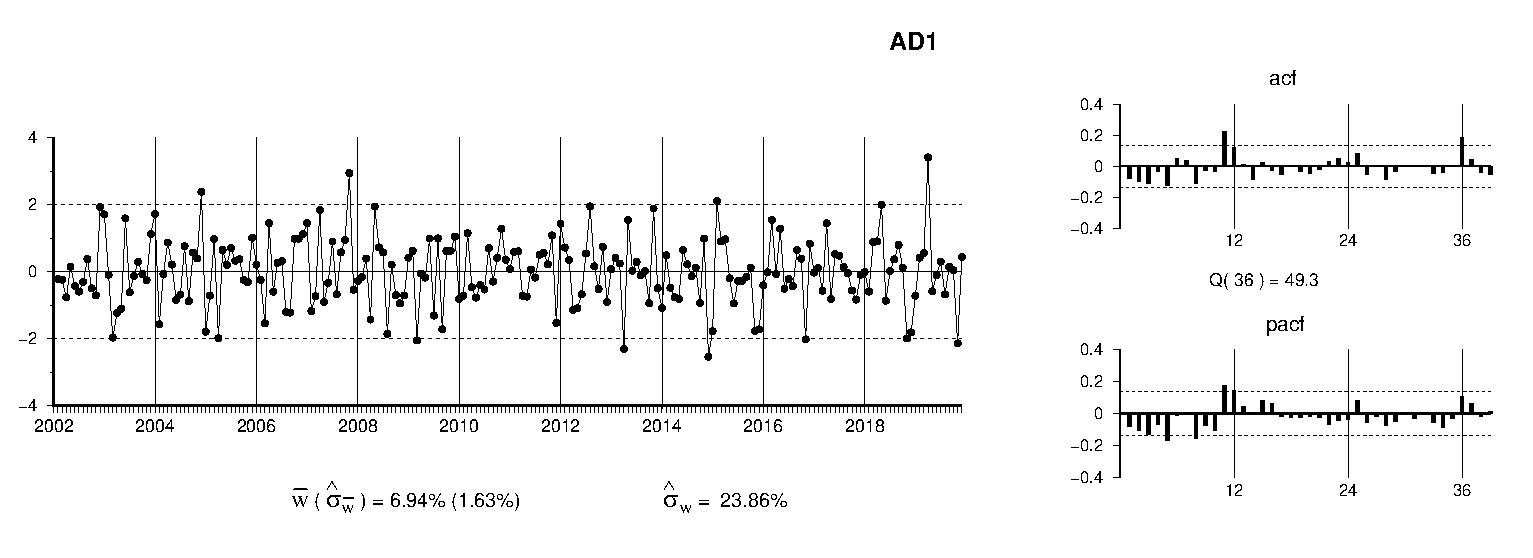
\includegraphics[scale=1]{AD1.eps}
\begin{footnotesize}
$\deter$ \\ 
 $ \arr 
\nrdiff 
\ifadf \mathsf{N_t} 
 = \mathsf{AD1_{t}} ; \quad 
\hat{\sigma}_{\mathsf{AD1}}=  \mathsf{ 0.25 } \%  $ 

\bigskip 
\begin{multicols}{2}{ 
\begin{tabular}{ccc}
\hline  Obs.  &  Date &  Std. Val. \\ 
\hline 
                       35 &       12/2004 &          2.38 \vspace{-.12in} \\  
                       70 &       11/2007 &          2.95 \vspace{-.12in} \\  
                       86 &        3/2009 &         -2.05 \vspace{-.12in} \\  
                      135 &        4/2013 &         -2.31 \vspace{-.12in} \\  
                      155 &       12/2014 &         -2.54 \vspace{-.12in} \\  
                      157 &        2/2015 &          2.11 \vspace{-.12in} \\  
                      178 &       11/2016 &         -2.02 \vspace{-.12in} \\  
                      207 &        4/2019 &          3.42 \vspace{-.12in} \\  
                      214 &       11/2019 &         -2.14 \vspace{-.12in} \\  
 \end{tabular} 
\\ 
 \columnbreak 
 \singlespacing 
 \underline{\textbf{Comments:}} \\ 
 \bigskip       

% \underline{Action:} 
 } 
\end{multicols} 

\end{footnotesize}
\end{flushleft}
\end{document}
